\chapter{The Value of a Reliable Description}\label{ch:specificity}

For $p=1$, the Bayesian predictor uses the posterior mean of $w^\top x$. Its risk is the expected trace of the posterior covariance of $w$. Let $X_n$ contain the demonstration inputs as rows and write $W_n=X_n^\top X_n$. Then
\begin{align*}
R^{\mathrm{demo}}(n)&=\E\operatorname{tr}(a_0^{-1}I_d+W_n)^{-1},\\
R^{\mathrm{desc}}_{p=1}(n)&=\E\operatorname{tr}(cI_d+W_n)^{-1}.
\end{align*}
The description replaces baseline precision $a_0^{-1}$ with $c$. Its predictive value is not, however, determined by this precision difference alone.

\begin{proposition}[Reliable descriptions]\label{prop:reliable}
Let $p=1$.
\begin{enumerate}[label=(\roman*),nosep,leftmargin=*]
\item With $r\in(0,1]$ fixed, $\ess_0\geq(1-r)d$, and $\ess_0\to(1-r)d$ as $a_0\to\infty$.
\item With positive integer $c$ fixed, $\ess_0\to c+d+1$ as $a_0\to\infty$.
\end{enumerate}
\end{proposition}

The two limits describe different regimes (proof in Section~\ref{app:specificity}). In the first, the description removes a fixed fraction of uncertainty in every direction. Each of the first $d$ demonstrations constrains one direction, so reducing variance across all directions can save approximately $(1-r)d$ demonstrations. In the second, the description retains a fixed absolute precision while the baseline prior becomes diffuse. Without a description, the limiting risk is $d/(n-d-1)$ for $n>d+1$ \citep{muirhead1982}; the description alone has risk $d/c$. These risks match at $n=c+d+1$. The integer restriction makes the crossing coincide with a measured count under linear interpolation.

This $d+1$ contribution reflects the cost of learning a $d$-dimensional task from random inputs. Matching average information would count only the added precision $c-a_0^{-1}$; matching predictive error also accounts for the random design. We refer to the additional contribution as the \emph{dimension term}. It is substantial when $c$ is small relative to $d$, whereas precision dominates when $c$ is large. This interpretation concerns the stated limits, rather than an exact additive formula for every finite $a_0$ and $n$.

The comparison with matching information can be made explicit in this limit. For a normal prior, the ESS of \citet{morita2008} is the ratio of the observation variance to the prior variance, so raising the baseline precision $a_0^{-1}$ to $c$ is worth $c-a_0^{-1}=(1-r)c$ demonstrations under their definition, at every $n$. With a diffuse baseline prior, $n$ demonstrations leave risk $d/(n-d-1)$, not the risk $d/n$ that their expected information would suggest. Setting $d/n$ equal to the description's risk $d/c$ gives $n=c$; setting $d/(n-d-1)$ equal to it gives $n=c+d+1$. The dimension term is the gap between the two.

\begin{figure}[t]
\centering
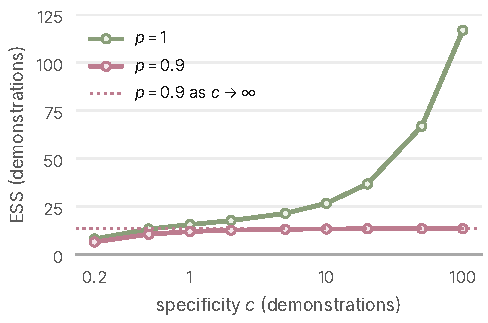
\includegraphics[width=0.75\textwidth]{ess_sq.pdf}
\caption[Reliability limits the benefit of greater specificity without demonstrations]{\textbf{Reliability limits the benefit of greater specificity without demonstrations.} Bayesian $\ess_0$ versus specificity $c$, for $p=1$ and $p=0.9$, at $d=16$ and $a_0=10$. The dotted line is the finite ceiling for $p=0.9$ as $c\to\infty$. Estimates use eight batches of $4{,}000$ prompts; standard errors are below $0.02$ demonstrations.}
\label{fig:ess}
\end{figure}

At $d=16$ and $a_0=10$, a reliable description with $c=1$ has ESS $15.6$, compared with the lower bound $(1-r)d=14.4$. Increasing $c$ to $100$ raises ESS to approximately $117$ (Figure~\ref{fig:ess}). As demonstrations accumulate, the dimension benefit disappears: $\ess_n\to c-a_0^{-1}$ (Corollary~\ref{cor:ess}). For example, after $100$ demonstrations the $c=1$ description is worth $1.1$ demonstrations, close to its added precision of $0.9$.

\paragraph{Coverage matters as well as precision.}
A description may constrain only $k<d$ directions. For any fixed precision $c>0$, its zero-demonstration ESS approaches $k$ as $a_0\to\infty$; increasing that fixed precision does not remove uncertainty in the other directions. With many demonstrations, its ESS instead approaches $k(c-a_0^{-1})/d$ (Proposition~\ref{prop:partial}). A precise partial description can therefore become more valuable as demonstrations resolve what it leaves unspecified. At $d=16$, $k=8$, and $c=100$, ESS increases from $8.1$ without demonstrations to $36$ with $100$ demonstrations (Table~\ref{tab:partial}).

\begin{table}[t]
\centering\small
\setlength{\tabcolsep}{3pt}
\caption[Demonstrations can increase the value of a precise partial description]{\textbf{Demonstrations can increase the value of a precise partial description.} Bayes-optimal ESS for a reliable description of $k$ of $d=16$ directions, with $a_0=10$. The case $k=16$ is a complete description. Each block reports ESS after $n$ demonstrations and its large-sample limit $(1-r)ck/d$. Estimates use eight batches of $2{,}000$ prompts; standard errors are at most $0.23$.}
\label{tab:partial}
\vspace{3pt}
\fittable{../paper/figs/partial_table.tex}
\end{table}

\section{Reliable Descriptions}\label{app:specificity}

\paragraph{Notation and risk.}
Write $\varepsilon = 1/a_0$, let $X_n\in\R^{n\times d}$ contain the demonstration inputs as rows, and set $W_n=X_n^\top X_n$. For $\kappa>0$, define
\[
R^{\kappa}(n)=\E\operatorname{tr}(\kappa I_d+W_n)^{-1}.
\]
Thus $R^{\mathrm{demo}}=R^{\varepsilon}$ and $R^{\mathrm{desc}}_{p=1}=R^c$. These identities follow from the posterior covariance under Gaussian linear regression. Conditional on the prompt, the posterior mean minimizes squared prediction error, and the independent query satisfies $\E[xx^\top]=I_d$. Averaging its conditional error $x^\top\Sigma x$ therefore gives $\E\operatorname{tr}\Sigma$.

Throughout the proofs, $d$ is a positive integer, $a_0>0$, $c\ge\varepsilon$, $r=1/(ca_0)\in(0,1]$, and $p\in[0,1]$. Noninteger sample sizes refer to linear interpolation between the risks at adjacent integers.

\paragraph{Wishart identities.}
We use three standard properties of $W_n$.
\begin{enumerate}[label=(W\arabic*),leftmargin=*]
    \item If $n<d$, then $W_n$ has rank $n$ almost surely. Consequently, $(\kappa I_d+W_n)^{-1}$ has $d-n$ eigenvalues equal to $1/\kappa$.
    \item If $n\ge d$ and $e$ is a fixed unit vector, then $(e^\top W_n^{-1}e)^{-1}\sim\chi^2_{n-d+1}$ \citep[Theorem~3.2.12]{muirhead1982}. Hence
    \[
    \E\operatorname{tr}W_n^{-1}=\frac{d}{n-d-1}\quad(n\ge d+2),
    \]
    whereas this expectation is infinite for $n=d$ and $n=d+1$.
    \item For fixed $d$, as $n\to\infty$,
    \[
    \E\operatorname{tr}W_n^{-2}=\frac{d}{n^2}+O(n^{-3}),
    \qquad
    \E\operatorname{tr}W_n^{-3}=O(n^{-3})
    \]
    \citep{vonrosen1988}.
\end{enumerate}
The Sherman--Morrison identity implies that an additional demonstration strictly decreases the expected trace of the posterior covariance. Thus $R^\kappa(n)$ is strictly decreasing, and (W2) implies that it tends to zero. Its linear interpolation is therefore continuous and strictly decreasing. In the correctly specified joint model, conditioning on the description cannot increase expected posterior variance, so $R^{\mathrm{desc}}(n)\le R^{\mathrm{demo}}(n)$ and the Bayes-optimal ESS is nonnegative.

\begin{proof}[Proof of Proposition~\ref{prop:reliable}]
A reliable description without demonstrations has risk
\[
R^{\mathrm{desc}}_{p=1}(0)=\frac{d}{c}=ra_0d.
\]

\emph{(i) Fixed variance reduction.}
By (W1), $R^\varepsilon(n)\ge(d-n)a_0$ for $n<d$; the inequality also holds trivially for $n\ge d$. Linear interpolation preserves this bound, so
\[
R^{\mathrm{demo}}(t)\ge(d-t)a_0\qquad(t\ge0).
\]
For $t<(1-r)d$, the right-hand side exceeds $ra_0d$. The matching sample size must therefore satisfy $\ess_0\ge(1-r)d$.

For every integer $n$,
\[
\frac{R^\varepsilon(n)}{a_0}
=\E\operatorname{tr}(I_d+a_0W_n)^{-1}
\longrightarrow(d-n)^+
\qquad\text{as }a_0\to\infty.
\]
Indeed, an eigenvalue $1/(1+a_0\lambda)$ is bounded by one and converges to the indicator of $\lambda=0$, so dominated convergence and the almost-sure rank of $W_n$ apply. The same limit holds at every real $t$ by interpolation. For fixed $r\in(0,1)$, the limiting curve crosses $rd$ at the unique point $t=(1-r)d$. Strict monotonicity then gives convergence of the crossing. For $r=1$, the description is uninformative and $\ess_0=0$ for every $a_0$, giving the same conclusion.

\emph{(ii) Fixed precision.}
For fixed $c>0$, the description risk $d/c$ is independent of $a_0$. As $a_0\to\infty$, monotone convergence, (W1), and (W2) give
\[
R^\varepsilon(n)\longrightarrow
\begin{cases}
+\infty,&n\le d+1,\\[2pt]
\displaystyle\frac{d}{n-d-1},&n\ge d+2.
\end{cases}
\]
If $c$ is a positive integer, the finite part of this limiting curve equals $d/c$ at the integer $n=c+d+1$. For every fixed point below this crossing the limiting risk is larger than $d/c$, and for every fixed point above it the limiting risk is smaller. The crossing of the interpolated finite-$a_0$ risk therefore converges to $c+d+1$. The integer condition ensures that the equality occurs at a grid point; linear interpolation does not in general preserve the same expression for noninteger $c$.
\end{proof}

\paragraph{Large-sample expansion.}
For fixed $d$ and $\kappa$, commuting $W_n$ with $\kappa I_d$ gives
\[
(\kappa I_d+W_n)^{-1}
=W_n^{-1}-\kappa W_n^{-2}
+\kappa^2W_n^{-2}(\kappa I_d+W_n)^{-1}.
\]
The final term is positive semidefinite and bounded above by $\kappa^2W_n^{-3}$. Using (W2) and (W3),
\begin{equation}\label{eq:extra}
R^\kappa(n)=\frac{d}{n-d-1}-\frac{\kappa d}{n^2}+O(n^{-3}).
\end{equation}
An additional demonstration reduces the leading term by $d/n^2+O(n^{-3})$. Thus a fixed change in prior precision and a fixed change in sample size affect risk at the same order. This observation underlies the large-$n$ ESS limits below.

\section{Partial Descriptions}\label{app:partial}

A reliable description may constrain only part of a task. Suppose it leaves a fraction $r$ of the baseline variance in $k<d$ directions and leaves the remaining $d-k$ directions unchanged. Its conditional prior precision is $c$ in the first set of directions and $\varepsilon=1/a_0$ in the second. Write
\[
\Lambda=\operatorname{diag}(cI_k,\varepsilon I_{d-k}).
\]
The prediction risk is $\E\operatorname{tr}(\Lambda+W_n)^{-1}$. Rotational invariance of $W_n$ means that the result depends on the number of constrained directions, not on their orientation.

\begin{proposition}[ESS of a partial description]\label{prop:partial}
Let $p=1$ and let $0\le k<d$ be an integer.
\begin{enumerate}[nosep]
    \item[(i)] As $a_0\to\infty$, $\ess_0\to(1-r)k$ with $r$ fixed, and $\ess_0\to k$ with $c$ fixed.
    \item[(ii)] For fixed $d$, $a_0$, and $c$, as $n\to\infty$,
    \[
    \ess_n\longrightarrow\frac{k}{d}(c-1/a_0)
    =\frac{k}{d}(1-r)c.
    \]
\end{enumerate}
\end{proposition}

In the broad-prior limit, the unconstrained directions dominate the initial error. Even an arbitrarily precise description of $k<d$ directions therefore replaces only about $k$ demonstrations when used alone. After many demonstrations, its value instead approaches the added precision averaged across all $d$ directions. These two limits permit complementarity: a sufficiently precise partial description can be worth more alongside demonstrations than by itself. The numerical example in Table~\ref{tab:partial} shows this effect. At $c=100$, a description of half of the $d=16$ directions has ESS $8.1$ without demonstrations and $36$ with $100$ demonstrations.

The large-sample limit exceeds $k$ about when $c-a_0^{-1}>d$, and this is when a partial description gains value as demonstrations accumulate. Between $0$ and $100$ demonstrations, a complete description at $c=100$ falls from $117$ to $109$, so demonstrations substitute for a complete description and complement a partial one. At $c=1$, ESS falls as demonstrations accumulate, whether the description is partial or complete.

\begin{proof}[Proof of Proposition~\ref{prop:partial}]
\emph{(i) No demonstrations.}
The description risk is
\[
\operatorname{tr}\Lambda^{-1}=(kr+d-k)a_0.
\]
Using $R^{\mathrm{demo}}(t)\ge(d-t)a_0$ gives $\ess_0\ge(1-r)k$. The normalized baseline risk converges to $(d-t)^+$, locally uniformly in $t$, by the integer limits and linear interpolation. With $r$ fixed, the normalized description risk is $d-(1-r)k$. With $c$ fixed, it is
\[
d-k+\frac{k}{ca_0}\longrightarrow d-k.
\]
Because $k<d$, both limiting levels are positive and have unique crossings, at $(1-r)k$ and $k$, respectively. Convergence of the crossings proves the claim. When the description leaves the prior unchanged, its ESS is identically zero.

\emph{(ii) Many demonstrations.}
Applying the resolvent identity twice gives
\[
(\Lambda+W_n)^{-1}
=W_n^{-1}-W_n^{-1}\Lambda W_n^{-1}
+W_n^{-1}\Lambda W_n^{-1}\Lambda(\Lambda+W_n)^{-1}.
\]
Rotational invariance implies
\[
\E W_n^{-2}=\frac{\E\operatorname{tr}W_n^{-2}}{d}I_d.
\]
The expected trace of the middle term is therefore
$\operatorname{tr}(\Lambda)/n^2+O(n^{-3})$ by (W3). To bound the remainder, use $|\operatorname{tr}(MB)|\le\|M\|_{\mathrm{op}}\operatorname{tr}B$ for $B\succeq0$, together with $(\Lambda+W_n)^{-1}\preceq W_n^{-1}$. Its absolute trace is at most
\[
\|\Lambda\|_{\mathrm{op}}^2\|W_n^{-1}\|_{\mathrm{op}}^2\operatorname{tr}W_n^{-1}
\le d\|\Lambda\|_{\mathrm{op}}^2\operatorname{tr}W_n^{-3},
\]
whose expectation is $O(n^{-3})$. Consequently,
\[
\E\operatorname{tr}(\Lambda+W_n)^{-1}
=\frac{d}{n-d-1}-\frac{\operatorname{tr}\Lambda}{n^2}+O(n^{-3}).
\]
Matching this expansion to the baseline risk, as in Corollary~\ref{cor:ess}(ii), gives
\[
\ess_n\longrightarrow\frac{\operatorname{tr}\Lambda-d\varepsilon}{d}
=\frac{k(c-\varepsilon)}{d}.
\]
\end{proof}
The same expansion applies to any fixed Gaussian description precision $\Lambda\succeq\varepsilon I_d$ compatible with the baseline task distribution. Its large-sample ESS is the added precision averaged across directions, $(\operatorname{tr}\Lambda-d\varepsilon)/d$.
